\documentclass{article}

\PassOptionsToPackage{numbers,compress}{natbib}
\usepackage[preprint]{Styles/neurips_2025}
\usepackage[utf8]{inputenc}
\usepackage[T1]{fontenc}
\usepackage{hyperref}
\usepackage{url}
\usepackage{booktabs}
\usepackage{graphicx}
\usepackage{amsmath}
\usepackage{microtype}
\usepackage{xcolor}

\title{Can Pre-trained Facial Expression Representations Predict Penalty Shootout Outcomes Beyond Match Context?}

\author{%
  XunZhi Cai \\
  \texttt{xcai166@connect.hkust-gz.edu.cn}
}

\newcommand{\prank}{\texttt{pooled\_rank}}
\newcommand{\fer}{\textsc{fer}}

\begin{document}

\maketitle

\begin{abstract}
This study asks whether pre-kick facial representations add predictive information beyond match context in penalty shootout. I study 40 shootouts, 412 kicks, and 385 valid face samples, comparing context-only, FER, ImageNet-control, fine-tuned, and fusion models under match-disjoint five-fold evaluation, ten split seeds, and permutation tests. No FER-only, fine-tuned, or fused model shows stable incremental value. Context logistic regression has weak, non-significant ranking ability. Results are limited to the present sample size, broadcast quality, and do not infer internal emotion.
\end{abstract}

\section{Introduction}

Penalty shootout is one of the most classic events in football. It turns a match outcome into a sequence of discrete decisions. Every player selected to take a penalty kick bears immense pressure—a strain often captured in the close-up shots of their faces during the broadcast. This background offers a possibility of event-level visual prediction. Therefore, I wonder whether a pretrained facial expression recognition (FER) representation adds information beyond historical penalty performance and match context.

The transfer setting is difficult. FER models are trained on expression datasets with different image distributions and label assumptions, while penalty-shootout footage collected in this study is compressed, low-resolution, and affected by many factors. To conduct a reasonable study, I applied Efficient Net trained on Affect Net dataset and used validation methods that ignores such dependence \citep{mollahosseini2019,tan2019,roberts2017,varma2006}.

In this project, I compare context-only models with frozen and fine-tuned FER representations, emotion probabilities, generic ImageNet features, and late fusion. The project contributes a completely new and well-developed dataset of penalty shootouts with facial crops of players, a leakage-controlled pre-kick pipeline, a match-disjoint comparison across representation and fusion choices, and a negative-result analysis with permutation tests, cluster bootstrap intervals. But still, the conclusion is a calibrated feasibility result for low-resolution broadcast footage.

\section{Related Work}

Facial-expression recognition (FER) depends on both the supervision used to train the encoder and the architecture used to represent the face. AffectNet addresses the first problem by providing a large in-the-wild corpus rather than a small collection of posed laboratory expressions \citep{mollahosseini2019}. The dataset contains more than one million Internet face images collected with emotion-related queries, of which 450,000 were manually annotated by human experts. Its annotations cover neutral and seven discrete expression categories, continuous valence and arousal, and face occlusion. Therefore, AffectNet is a diverse training resource and a shared label space for learning facial-appearance representations under variation in pose, lighting, resolution, and background. In this study, AffectNet-based FER pretraining supplies the source-domain supervision before any penalty-shootout sample is used.

EfficientNet addresses a different problem. Tan and Le propose a compound model-scaling method that increases network depth, width, and input resolution together according to a fixed scaling rule, rather than tuning one dimension in isolation \citep{tan2019}. They use this scaling principle to construct the EfficientNet model family, which is designed to improve the accuracy--efficiency trade-off of convolutional networks. Our main FER arm, \texttt{enet\_b0\_8\_best\_vgaf}, instantiates this transfer chain with an EfficientNet-B0 backbone. The underlying emotional CNN is trained on AffectNet's eight expression classes, while this checkpoint is the model variant selected for downstream performance on the VGAF video benchmark \citep{savchenko2022efficient,sharma2019vgaf}. It produces a 1,280-dimensional intermediate embedding together with eight emotion probabilities, both of which are evaluated in this paper. The ImageNet control uses the same general backbone family with generic visual pretraining \citep{deng2009}, so the comparison targets the value of expression-oriented pretraining rather than a difference in architecture or capacity.

The evaluation follows work on structured cross-validation. Grouped validation prevents observations from the same higher-level unit from being split across training and test, and nested model selection reduces selection bias \citep{roberts2017,varma2006}. I apply these principles at the match level and add cluster bootstrap intervals for auxiliary metrics.

\section{Methodology}

\subsection{Task and dataset}

Each observation is one penalty-shootout kick with a binary label. The final collection contains 40 matches and 412 recorded kicks. The preprocessing pipeline retained 385 valid observations, including 278 goals and 107 misses. Twenty-seven kicks were excluded because no qualified face frame was available. The videos are mainly 360p broadcast recordings. A candidate face was accepted only from a time window before ball contact. In addition, a table of kicks' context is included in the dataset which contains information like round number, scores for each round and historical performance of each player. The dataset can be found in my published github repository.(https://github.com/Grass456/Penalty-shoot-and-Expression)

\subsection{Preprocessing and features}

The visual branch selects a face crop, caches FER emotion probabilities and an intermediate embedding, and applies a linear downstream classifier. The main context branch uses six pre-kick variables constructed from context table. They encode temporally truncated historical penalty performance, round and kick order, sudden-death status, and the score before the kick, together with indicators for missing history. Historical statistics are computed only from completed seasons before the match date.

\subsection{Model families}

The core comparison includes a majority baseline, B1v2 context logistic regression, B2v2 context MLP, B3 emotion-probability classifiers, M1 frozen FER embeddings, B4 ImageNet embeddings, M2 partial FER fine-tuning, M3v2 frozen FER plus context, and M4 logit fusion. The ImageNet control uses a generic visual representation rather than an expression-specific encoder \citep{deng2009}. The context and FER branches are trained separately in the main fusion experiment. The fusion layer combines standardized branch logits with three fitted parameters. This design keeps the two branches attributable, while leaving higher-dimensional feature interaction for future work. Figure~\ref{fig:pipeline} summarizes the resulting information flow.

For a context vector $x_i$, the logistic baseline estimates $p_i=\sigma(\beta^{\top}x_i+b)$. In the fusion arms, standardized branch logits are combined as
\begin{equation}
\ell_i = w_f z^{\mathrm{FER}}_i + w_c z^{\mathrm{ctx}}_i + b,
\qquad p_i=\sigma(\ell_i),
\end{equation}
with the three fusion parameters fitted on the inner validation split.

\begin{figure}[t]
\centering
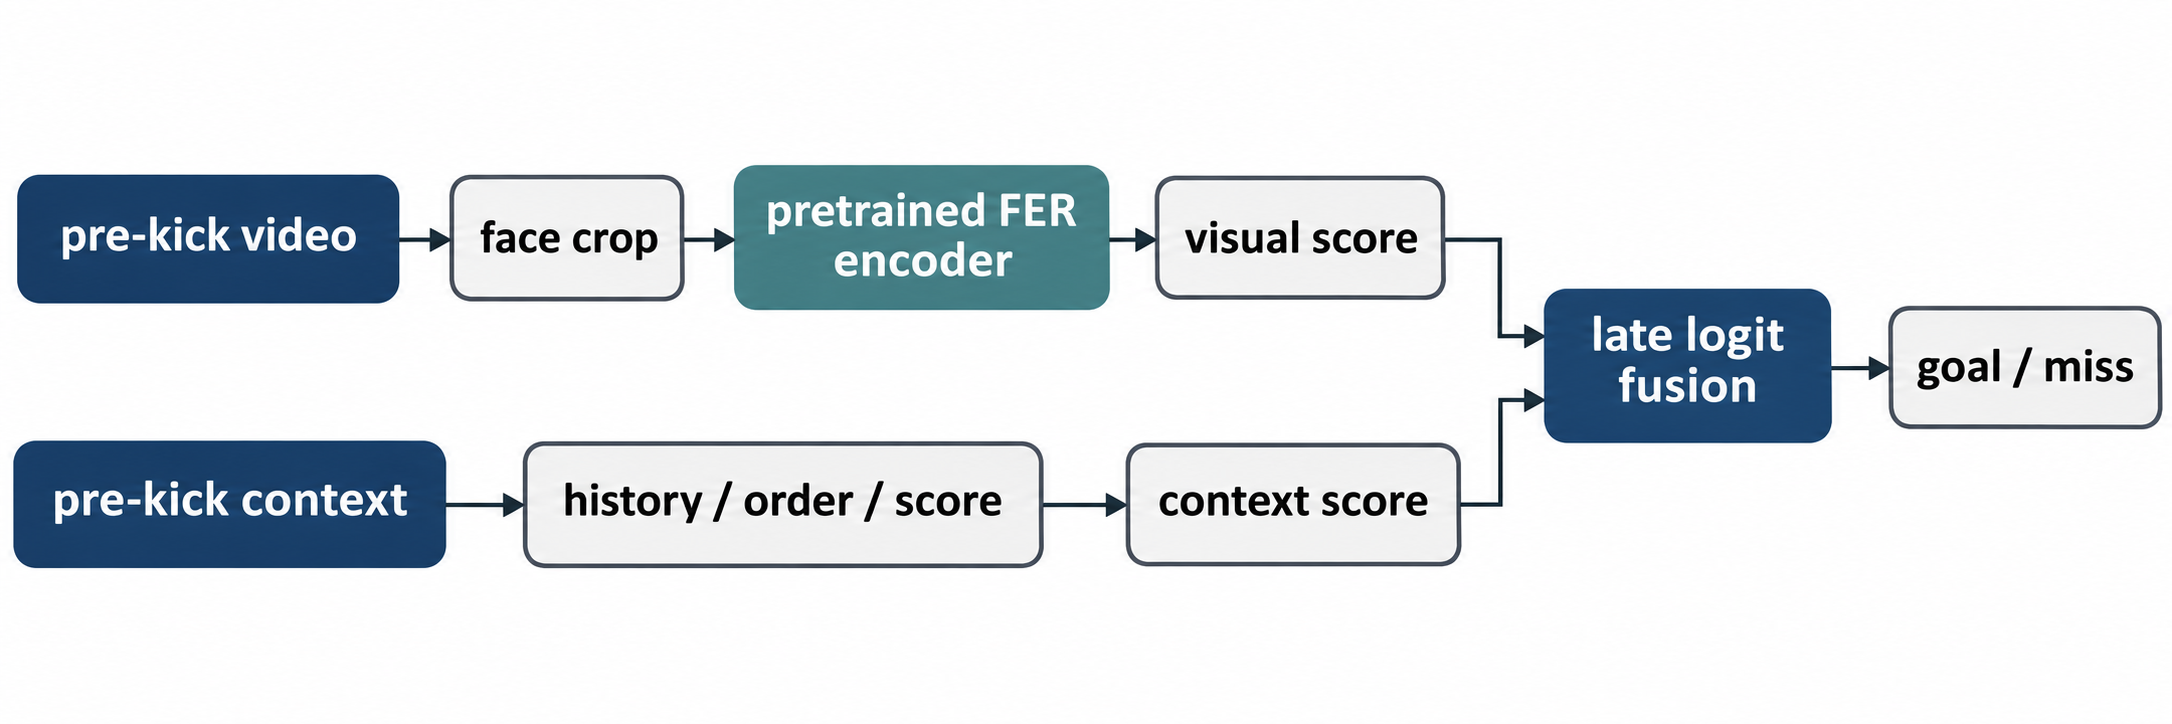
\includegraphics[width=0.99\columnwidth]{figures/fusion_pipeline.png}
\caption{Leakage-controlled fusion pipeline. All inputs are available before ball contact.}
\label{fig:pipeline}
\end{figure}

\subsection{Evaluation protocol}

The primary evaluation uses stratified grouped five-fold cross-validation with \texttt{match\_id} as the group. No match contributes kicks to both training and test partitions. An inner grouped validation split is used for early stopping and fold-local preprocessing. Ten split seeds quantify training and partition variation. The main statistic is \prank, obtained by converting predictions to within-fold ranks $r_{ij}=(\operatorname{rank}(p_{ij})-0.5)/n_j$ before pooling them across held-out events and computing the goal-versus-miss ranking AUC. This removes arbitrary probability-scale differences between folds while preserving within-fold ordering.

For each arm, 200 full-label permutation refits form a null distribution for \prank \citep{good2005}. I report the ten-seed mean and standard deviation together with the right-tail permutation probability. Secondary metrics are AUROC, AUPRC, goal-class F1 at threshold 0.5, balanced accuracy, Brier score, and log loss. Goal-class F1 uses the observed 72.2\% goal rate and is therefore auxiliary. For uncertainty intervals, 2,000 bootstrap resamples draw complete matches with replacement, following the cluster principle introduced by Efron \citep{efron1979}. All scaling, history shrinkage, early stopping, and model selection are fit inside the corresponding training or validation partitions.

\section{Empirical Analysis}

\subsection{Main results}

Table~\ref{tab:main} summarizes the principal arms. Context LR is closest to the permutation threshold, but its $p=.060$ does not meet the prespecified criterion. Frozen FER, ImageNet, fusion, fine-tuning, and both M4 variants all fail their corresponding tests.

\begin{table}[t]
\caption{Core results over ten split seeds. The primary statistic is \prank. F1 intervals use 2,000 match-cluster bootstrap resamples. The dagger marks the degraded single-seed paired permutation protocol used for M2 and M4.}
\label{tab:main}
\centering
\small
\setlength{\tabcolsep}{3.2pt}
\begin{tabular}{lccc}
\toprule
Arm & \prank mean $\pm$ SD & test $p$ & F1 mean $\pm$ SD [95\% CI]\\
\midrule
B1v2 context LR & .553 $\pm$ .017 & .060 & .838 $\pm$ .001 [.803,.871]\\
M1 frozen FER & .467 $\pm$ .028 & .821 & .780 $\pm$ .013 [.746,.811]\\
B4 ImageNet & .464 $\pm$ .021 & .831 & .780 $\pm$ .009 [.750,.812]\\
M3v2 fused & .467 $\pm$ .028 & .811 & .781 $\pm$ .012 [.746,.811]\\
M2 partial FT & .488 $\pm$ .024 & .475$^{\dagger}$ & .837 $\pm$ .004 [.802,.870]\\
M4\_lr & .505 $\pm$ .022 & .881$^{\dagger}$ & .834 $\pm$ .004 [.798,.868]\\
M4\_mlp & .491 $\pm$ .024 & .297$^{\dagger}$ & .833 $\pm$ .005 [.798,.867]\\
\bottomrule
\end{tabular}
\end{table}

Figure~\ref{fig:main-results} shows the complete comparison. The FER--ImageNet difference is only $+0.003$ ($p=.483$), and adding FER to context changes the ranking by $-0.086$. F1 is auxiliary because goals are the common class, whereas \prank is the primary ranking measure.

\begin{figure*}[t]
\centering
\includegraphics[width=\textwidth]{figures/fig1_main_results.pdf}
\caption{Main ranking results and preregistered paired comparisons. Error bars in the left panel show split-seed standard deviation. The shaded regions show the permutation-null mean to 95th-percentile range.}
\label{fig:main-results}
\end{figure*}

\subsection{Robustness and ablations}

The random-event split does not show inflation relative to match-disjoint evaluation. Random-minus-matched differences range from $-0.010$ to $-0.003$, with no paired test passing. Context ablations, the \texttt{minus\_history} recheck, and the quality-subset analysis likewise produce no stable change in the main conclusion.

\subsection{Additional representation and temporal analyses}
In addition, I compare eight-emotion embedding with continuous Valence-arousal embedding and single-frame inputs with multi-frame inputs.

The VA multi-task embedding has mean \prank .490 versus .467 for the eight-emotion FER embedding, with a paired difference of $+0.024$ and $p=.164$. Valence--arousal supervision therefore does not yield a reliable improvement. On the same 356-observation subset, multi-frame mean aggregation reaches .494 versus .449 for single-frame input, with $\Delta=+0.045$ and $p=.134$. This direction is consistent with reduced frame-level noise, but it is not statistically stable.

\section{Discussion}

Frozen FER and ImageNet representations obtain nearly identical ranking performance (.467 versus .464), and neither exceeds its permutation null. Because the two arms use the same EfficientNet family and downstream evaluation, the result provides little evidence that expression-oriented pretraining contains more outcome-relevant information than generic visual pretraining. The representation can encode facial appearance useful for its source task while still being poorly aligned with a goal/miss label in compressed broadcast footage.

The context branch supplies only a weak reference. Context LR reaches .553 with $p=.060$, close to the detection boundary but still below the prespecified criterion. Adding FER lowers the ranking statistic, while partial fine-tuning and logit fusion do not recover an increment. These results suggest that the main bottleneck is the transfer of a pre-kick facial representation to the event label, rather than a missing optimization step in the downstream classifier.

The additional controls narrow the set of simple explanations. Valence--arousal supervision does not reliably improve the eight-emotion representation, and mean aggregation across frames does not produce a significant gain over a single frame. Changing the affect label space or averaging nearby observations therefore does not rescue the transfer signal. 

As for the limitation, the study uses only 40 matches and 385 valid samples from low-resolution broadcasts. The split is not player-disjoint, and the fusion model uses a restricted logit design. These constraints set the scope of the claim. Moreover, Facial features are statistical inputs for an observed outcome and are not measurements of private emotion or psychological condition \citep{barrett2019}.

\section{Conclusion}

This project tests whether a pretrained facial expression representation adds predictive information to penalty-shootout models beyond match context. Three findings define the result. Context provides weak, non-significant ranking ability. FER performs no better than a same-backbone ImageNet representation. Fine-tuning, fusion, valence--arousal supervision, and multi-frame averaging do not produce a stable incremental gain. The contribution is therefore a well-developed dataset of penalty-shootout, a leakage-controlled feasibility benchmark and a bounded negative finding. Future work can extend the scale of experiment and optimize the model in both parameters and architectures. In present study, we cannot find any signal of facial expression. But if it exists in the larger scale, it will be a significant finding in both sports science and psychology.

\bibliographystyle{plainnat}
\bibliography{references}

\clearpage
\appendix
\section{Extended results and reproducibility}

The complete arm list includes B1v2, B2v2, B3\_vgaf, B3\_b2\_7, M1, B4, M3v2, VAemb, single356, multimean, multiva2, M2, M4\_lr, M4\_mlp, M4\_lr\_tr, and M4\_mlp\_tr. The evaluation scripts record the folds, split seeds, permutation seeds, and deterministic initialization settings. Figures~\ref{fig:seed-stability} and~\ref{fig:signal-map} show the extended stability and quality-subset diagnostics.

\begin{figure}[h]
\centering
\includegraphics[width=0.92\linewidth]{figures/fig2_seed_stability.pdf}
\caption{Split-seed stability for the main and recheck seed sets.}
\label{fig:seed-stability}
\end{figure}

\begin{figure}[h]
\centering
\includegraphics[width=0.92\linewidth]{figures/fig3_signal_map.pdf}
\caption{Descriptive context effects and the quality-subset comparison.}
\label{fig:signal-map}
\end{figure}

All of the content can be found in my published repository. (https://github.com/Grass456/Penalty-shoot-and-Expression)

\subsection{Implementation details}

The context LR and FER LR arms use fold-local standardization and fixed regularization settings recorded in the evaluation scripts. The MLP arms use seeded initialization, early stopping on the inner validation split, and fold-local scaling. M2 unfreezes the last encoder stage and classification head with the recorded discriminative learning rates while keeping batch-normalization statistics frozen. M4 fits a three-parameter standardized-logit fusion layer. The bootstrap uses 2,000 match-level resamples and percentile limits. The label permutation analyses refit the full evaluation pipeline for 200 permutations unless a report explicitly records the degraded single-seed protocol.

\subsection{Scope deviations}

The final analysis does not include venue status or competition category, and it does not execute the planned attribution analysis. The quality subset uses complete-match filtering rather than independent sample filtering. M4 uses logit fusion instead of the originally planned high-dimensional feature interaction model. These deviations are recorded in the project summary and delimit the claims made in the main text.

\end{document}
